% Copyleft 2010 by Walter Vargas <walter@covetel.com.ve>
% Presentación de Peribeco - Primera Fase. 

\documentclass{beamer}
\usepackage{listings}
\lstset{language=Perl}

% Configuración de la apariencia. 

\usetheme{Szeged}
\usecolortheme{beaver}
\usefonttheme[onlylarge]{structurebold}
\setbeamerfont*{frametitle}{size=\normalsize,series=\bfseries}

%\setbeamertemplate{navigation symbols}{}

% Paquetes
\usepackage[utf8]{inputenc}
\usepackage[spanish]{babel}

% Titulo
\title[Perl 01] {Curso de Perl Nivel Básico}
\author[Walter Vargas]{ info@covetel.com.ve \inst{1}}
\institute[covetel.com.ve]{ \inst{1} Cooperativa Venezolana de Tecnologías Libres R.S. }
\date[1 de Enero de 2011]{1 de Enero de 2011}

\begin{document}

\begin{frame}
  \titlepage
\end{frame}

\begin{frame}{Sobre Perl} % (fold)
Perl tiene unos 23 años hasta ahora. El lenguaje ha evolucionado desde una
herramienta simple para la administración de sistemas tomando cosas de shell
scripting y C (Perl 1) hasta convertirse en un poderoso lenguaje de propósito
general (Perl 5), consistente, coherente, cambiando el paradigma de
programación en general con la intensión de mantenerse por otros 25 años. (Perl
6) 
\end{frame}

\begin{frame}{Porque Larry creo Perl ?} % (fold)
Larry crea Perl a mediados de 1980,  cuando intentaba producir reportes sobre 
la información ordenada jerárquicamente en archivos de  la red de noticias 
USENET para un sistema de reporte de bugs,  y awk no dio la talla. Entonces
Larry, como buen programador perezoso que es,  decide hacer una herramienta que
pueda usar para resolver este problema y que pueda volver a usar para otro
problema similar en otro lugar,  en otro tiempo. 
\end{frame}

\begin{frame}{La mascota} % (fold)
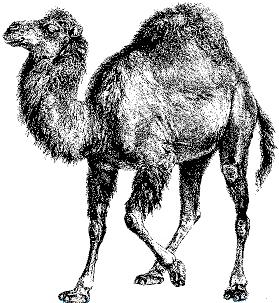
\includegraphics[scale=1]{imgs/dromedario.jpg}
\end{frame}

\begin{frame}{Características principales de Perl} % (fold)
\begin{itemize}
    \item Perl es Fácil
    \item Perl es casí ilimitado
    \item Perl es sobre todo rápido 
    \item Perl es un poco feo  
\end{itemize}
\end{frame}

\begin{frame}{Perl es Fácil} % (fold)
Cuando nos referimos que Perl es fácil, hablamos de que es fácil de usar, no es
especialmente fácil de aprender. Si usted conduce un carro, que paso semanas o
meses aprendiendo a conducir, entonces luego va a ser fácil de conducir. De
igual manera cuando pase la misma o mas cantidad de horas aprendiendo Perl,
entonces despues va a ser muy fácil de usar.  

\end{frame}

\begin{frame}{Perl es casí ilimitado} % (fold)
Hay muy pocas cosas que no podrás hacer con Perl. Seguramente usted no deseará
escribir un controlador de algún dispositivo de interrupción a nivel de
micro-kernel (A pesar de que ya alguien hizo esto). Pero la mayoria de las
cosas que la gente común y no tan común necesita,  la mayoria del tiempo son
buenas tareas para Perl, desde scripts muy pequeños, hasta aplicaciones de
nivel industrial. 
\end{frame}

\begin{frame}{Perl es sobre todo rápido} % (fold)
Esto es porque no hay nadie en el desarrollo que no lo utilice, de modo que
entonces todos queremos que Perl sea rápido. Si alguien quiere añadir una nueva
característica que sea genial, pero que introduzca lentitud a otros aspectos,
es casí seguro que Larry va a rechazar la nueva característica hasta que no se
encuentre una manera de escribirla de manera eficiente. 
\end{frame}

\begin{frame}{Perl es un poco feo} % (fold)
Esto es cierto, el camello se ha convertido en el simbolo de Perl, desde la
cubierta del legendario libro {\bf The Camel Book}, conocido tambien como
{\bf Programming Perl by Larry Wall, Tom Christianesen,  and Jon Orwant}. 
Los camellos tambien son un poco feos, pero trabajan duro, incluso en
condiciones difíciles. Los camellos siempre están ahí siempre para hacer el
trabajo a pesar de todas las dificultades, incluso cuando se ven y huelen mal e
incluse le escupen. Perl es un poco así.
\end{frame}

\begin{frame}{¿ Perl es fácil o difícil ?} % (fold)
Perl es fácil de usar, pero a veces difícil de aprender. Esto por su puesto es
una gereralización. En el diseño de Perl, Larry tuvo que hacer muchas
consideraciones. Cuando ha tenido la oportunidad de hacer algo más fácil para
el programador a costa de ser más difícil para el estudiante, ha decidido casi
todo el tiempo a favor del programador. Esto es así, porque usted va a aprender
Perl una sola vez, pero lo vas a usar una y otra vez. Perl posee cualquier
cantidad de comodidades que le permiten al programador ahorrar tiempo. Por
ejemplo,  la mayoria de las funciones tienen un valor predeterminado,  con
frecuencia,  el valor por defecto es justamente la manera en la que usted desea
usar la función. 
\end{frame}

\begin{frame}{¿ Como se hizo Perl tan popular ?} % (fold)
Despues de jugar un rato con Perl, agregando cosas aquí y allá, Larry se lanzó
a la comunidad de lectores de la Usenet,  comunmente conocidad como B<La Red>.
Los usuarios de esta flota fugitiva que trabajaban en sistemas en todo el
mundo (decenas de miles de ellos), le dieron retroalimentación, pidiendo a
Larry, maneras de hacer esto, aquello o lo otro, muchos de los cuales Larry
nunca había imaginado en su poco manejo de Perl. 

Pero como resultado, Perl creció, y creció y creció. Creció en características.
Creció en portabilidad. 

\end{frame}

\begin{frame}{¿ Que esta pasando con Perl ahora ? } % (fold)
Durante estos días, Larry Wall no escribe código, pero el sigue guiando el
desarrollo y toma las desiciones importantes. Perl es mayormente mantenido por
un grupo de resistentes y valientes personas llamadas B<The Perl 5 Porters>.
Puede suscribirse a la lista de correo en L<perl5-porters@perl.org> para seguir
el trabajo de esta gente y sus debates. Al momento de escribir esta
documentación,  muchas cosas estan pasando con Perl. Durante los últimos años,
muchas personas han estado trabajando en la próxima versión de Perl: Perl 6.
\end{frame}

\begin{frame}{¿ Va a estar Perl 5 obsoleto ?} % (fold)
No tire a un lado Perl 5, este sigue siendo la versión actual y estable. No se
espera una version estable de Perl 6 durante un rato largo. Perl 5 hace todo lo
de siempre, y siempre sera así. Perl 5 no va a desaparecer cuando Perl 6 salga.
Y la gente puede seguir usando Perl 5 durante muchos años mas. 
\end{frame}
% section Introducción (end)

\begin{frame}{¿ Que es CPAN ?} % (fold)
CPAN es {\bf Comprehensive Perl Archive Network}, su primera parada para Perl.
Posee el código fuente de Perl, listo para instalar y los {\bf ports} para 
todos los sistemas no Unix, ejemplos, documentación, y extensiones
del lenguaje. 

CPAN es replicado en cientos de máquinas al rededor del mundo, comenzando en
{\bf http://search.cpan.org} o {\bf http://kobesearch.cpan.org} para navegar 
o buscar un paquete. Si no tienes acceso a la red, todo CPAN puede caber 
en 8 o 10 GB.

\end{frame}

\begin{frame}{¿ Como hacer un programa en Perl ?} % (fold)
Ya es tiempo de hacer esta pregunta (aunque usted no la halla hecho aun), Los
programas de Perl son archivos de texto plano, usted puede crearlos y editarlos
en su editor de textos preferido,  yo personalmente prefiero {\bf VIM}. 
(Usted no 
necesita entornos de desarrollo especiales, aunque hay disponibles editores
comerciales de varios proveedores. Nunca hemos utilizado uno de estos lo
suficiente como para recomendarlo). Por lo general debería usar un editor de
texto pensado para programadores, en lugar de un editor de textos
convencional. ¿ Cual es la diferencia ? Bueno, un editor pensado para
programadores le va a permitir hacer cosas que necesitan los programadores,
como sangrado automático o subrayado de bloques de código, o indicar
automáticamente la llave de cierre de un bloque de código. 
La página del manual {\bf perlfaq3} tiene una
lista de otros editores que también pueden usarse.
\end{frame}

\begin{frame}{Evaluación Inicial} % (fold)
    Solicite al instructor la evaluación inicial.
\end{frame}

\end{document}
